\begin{pa} \label{PA:1.2}
Suppose that $g$ is the function given by the graph below.  Use the graph to answer each of the following questions. 
\ba
	\item Determine the values $g(-2)$, $g(-1)$, $g(0)$, $g(1)$, and $g(2)$, if defined.  If the function value is not defined, explain what feature of the graph tells you this.
	\item For each of the values $a = -1$, $a = 0$, and $a = 2$, complete the following sentence: ``As $x$ gets closer and closer (but not equal) to $a$, $g(x)$ gets as close as we want to \underline{\hspace{0.3in}}.''
	\item What happens as $x$ gets closer and closer (but not equal) to $a = 1$?  Does the function $g(x)$ get as close as we would like to a single value?
\ea

\begin{figure}[h]
\begin{center}
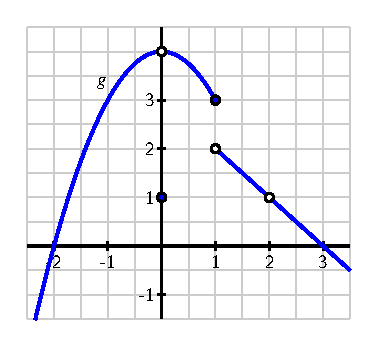
\includegraphics{figures/1_2_PA1.eps} 
\caption{Graph of $y = g(x)$ for Preview Activity~\ref{PA:1.2}.} \label{F:1.2.PA1}
\end{center}
\end{figure}

\end{pa} \afterpa